%%========================================================================
%% LaTeX sjabloon voor stage/projectrapport of bachelorproef
%%  HoGent Bedrijf en Organisatie
%%========================================================================

%%========================================================================
%% Preamble
%%========================================================================

\documentclass[pdftex,a4paper,12pt,twoside]{report}

% XXX: Let op: dit sjabloon is gemaakt om dubbelzijdig af te drukken
% Voor enkelzijdig, verwijder ``twoside'' hierboven.

%%---------- Extra functionaliteit ---------------------------------------

\usepackage[utf8]{inputenc}  % Accenten gebruiken in tekst (vb. é ipv \'e)
\usepackage{amsfonts}        % AMS math packages: extra wiskundige
\usepackage{amsmath}         %   symbolen (o.a. getallen-
\usepackage{amssymb}         %   verzamelingen N, R, Z, Q, etc.)
\usepackage[dutch]{babel}    % Taalinstellingen: woordsplitsingen,
                             %  commando's voor speciale karakters
                             %  ("dutch" voor NL)
\usepackage{eurosym}         % Euro-symbool €
\usepackage{geometry}
\usepackage{graphicx}        % Invoegen van tekeningen
\usepackage[pdftex,bookmarks=true]{hyperref}
                             % PDF krijgt klikbare links & verwijzingen,
                             %  inhoudstafel
\usepackage{listings}        % Broncode mooi opmaken
\usepackage{multirow}        % Tekst over verschillende cellen in tabellen
\usepackage{rotating}        % Tabellen en figuren roteren
\usepackage{natbib}          % Betere bibliografiestijlen
\usepackage{fancyhdr}        % Pagina-opmaak met hoofd- en voettekst

\usepackage[T1]{fontenc}     % Ivm lettertypes
\usepackage{lmodern}
\usepackage{textcomp}
\usepackage{subfiles}
\usepackage{subcaption}
\usepackage{caption}
\usepackage{dirtytalk}
\usepackage{minted}
\usepackage{epigraph}

%%---------- Layout ------------------------------------------------------

% hoofdingen, enz.
\pagestyle{fancy}
% enkel hoofdstuktitel in hoofding, geen sectietitel (vermijd overlap)
\renewcommand{\sectionmark}[1]{}

% lijn, wordt gebruikt in titelpagina
\newcommand{\HRule}{\rule{\linewidth}{0.5mm}}

% Leeg blad
\newcommand{\emptypage}{
\newpage
\thispagestyle{empty}
\mbox{}
\newpage
}

% Gebruik een schreefloos lettertype ipv het "oubollig" uitziende
% Computer Modern
\renewcommand{\familydefault}{\sfdefault}

% Commando voor invoegen Java-broncodebestanden (dank aan Niels Corneille)
% Gebruik: \codefragment{source/MijnKlasse.java}{Uitleg bij de code}
\newcommand{\codefragment}[2]{ \lstset{%
  language=java,
  breaklines=true,
  float=th,
  caption={#2},
  basicstyle=\scriptsize,
  frame=single,
  extendedchars=\true
}
\lstinputlisting{#1}}

%%---------- Documenteigenschappen ---------------------------------------
%% Vul dit aan met je eigen info:

% Je eigen naam
\newcommand{\student}{Dieter Vyncke}

% De naam van je lector, begeleider, promotor
\newcommand{\promotor}{Jens Buysse}

% De naam van je co-promotor
\newcommand{\copromotor}{Joeri Van Steen }

% De titel van het rapport/bachelorproef
\newcommand{\titel}{CMS bovenop PHP framework Laravel biedt het antwoord op de klant gefocuste CMS met behoud van de focus voor ontwikkelaars. 
Proof of concept.}



% Datum van indienen
\newcommand{\datum}{}

% Faculteit
\newcommand{\faculteit}{Faculteit Bedrijf en Organisatie}

% Soort rapport
\newcommand{\rapporttype}{Scriptie voorgedragen tot het bekomen van de graad van\\Bachelor in de toegepaste informatica}

% Academiejaar
\newcommand{\academiejaar}{2015-2016}

% Examenperiode
%  - 1e semester = 1e examenperiode
%  - 2e semester = 2e examenperiode
%  - tweede zit = 3e examenperiode
\newcommand{\examenperiode}{Tweede examenperiode}

%%========================================================================
%% Inhoud document
%%========================================================================

\begin{document}

%%---------- Front matter ------------------------------------------------
%% Het voorblad - Hier moet je in principe niets wijzigen.

\begin{titlepage}
  \newgeometry{top=2cm,bottom=1.5cm,left=1.5cm,right=1.5cm}
  \begin{center}

    \begingroup
    \rmfamily
    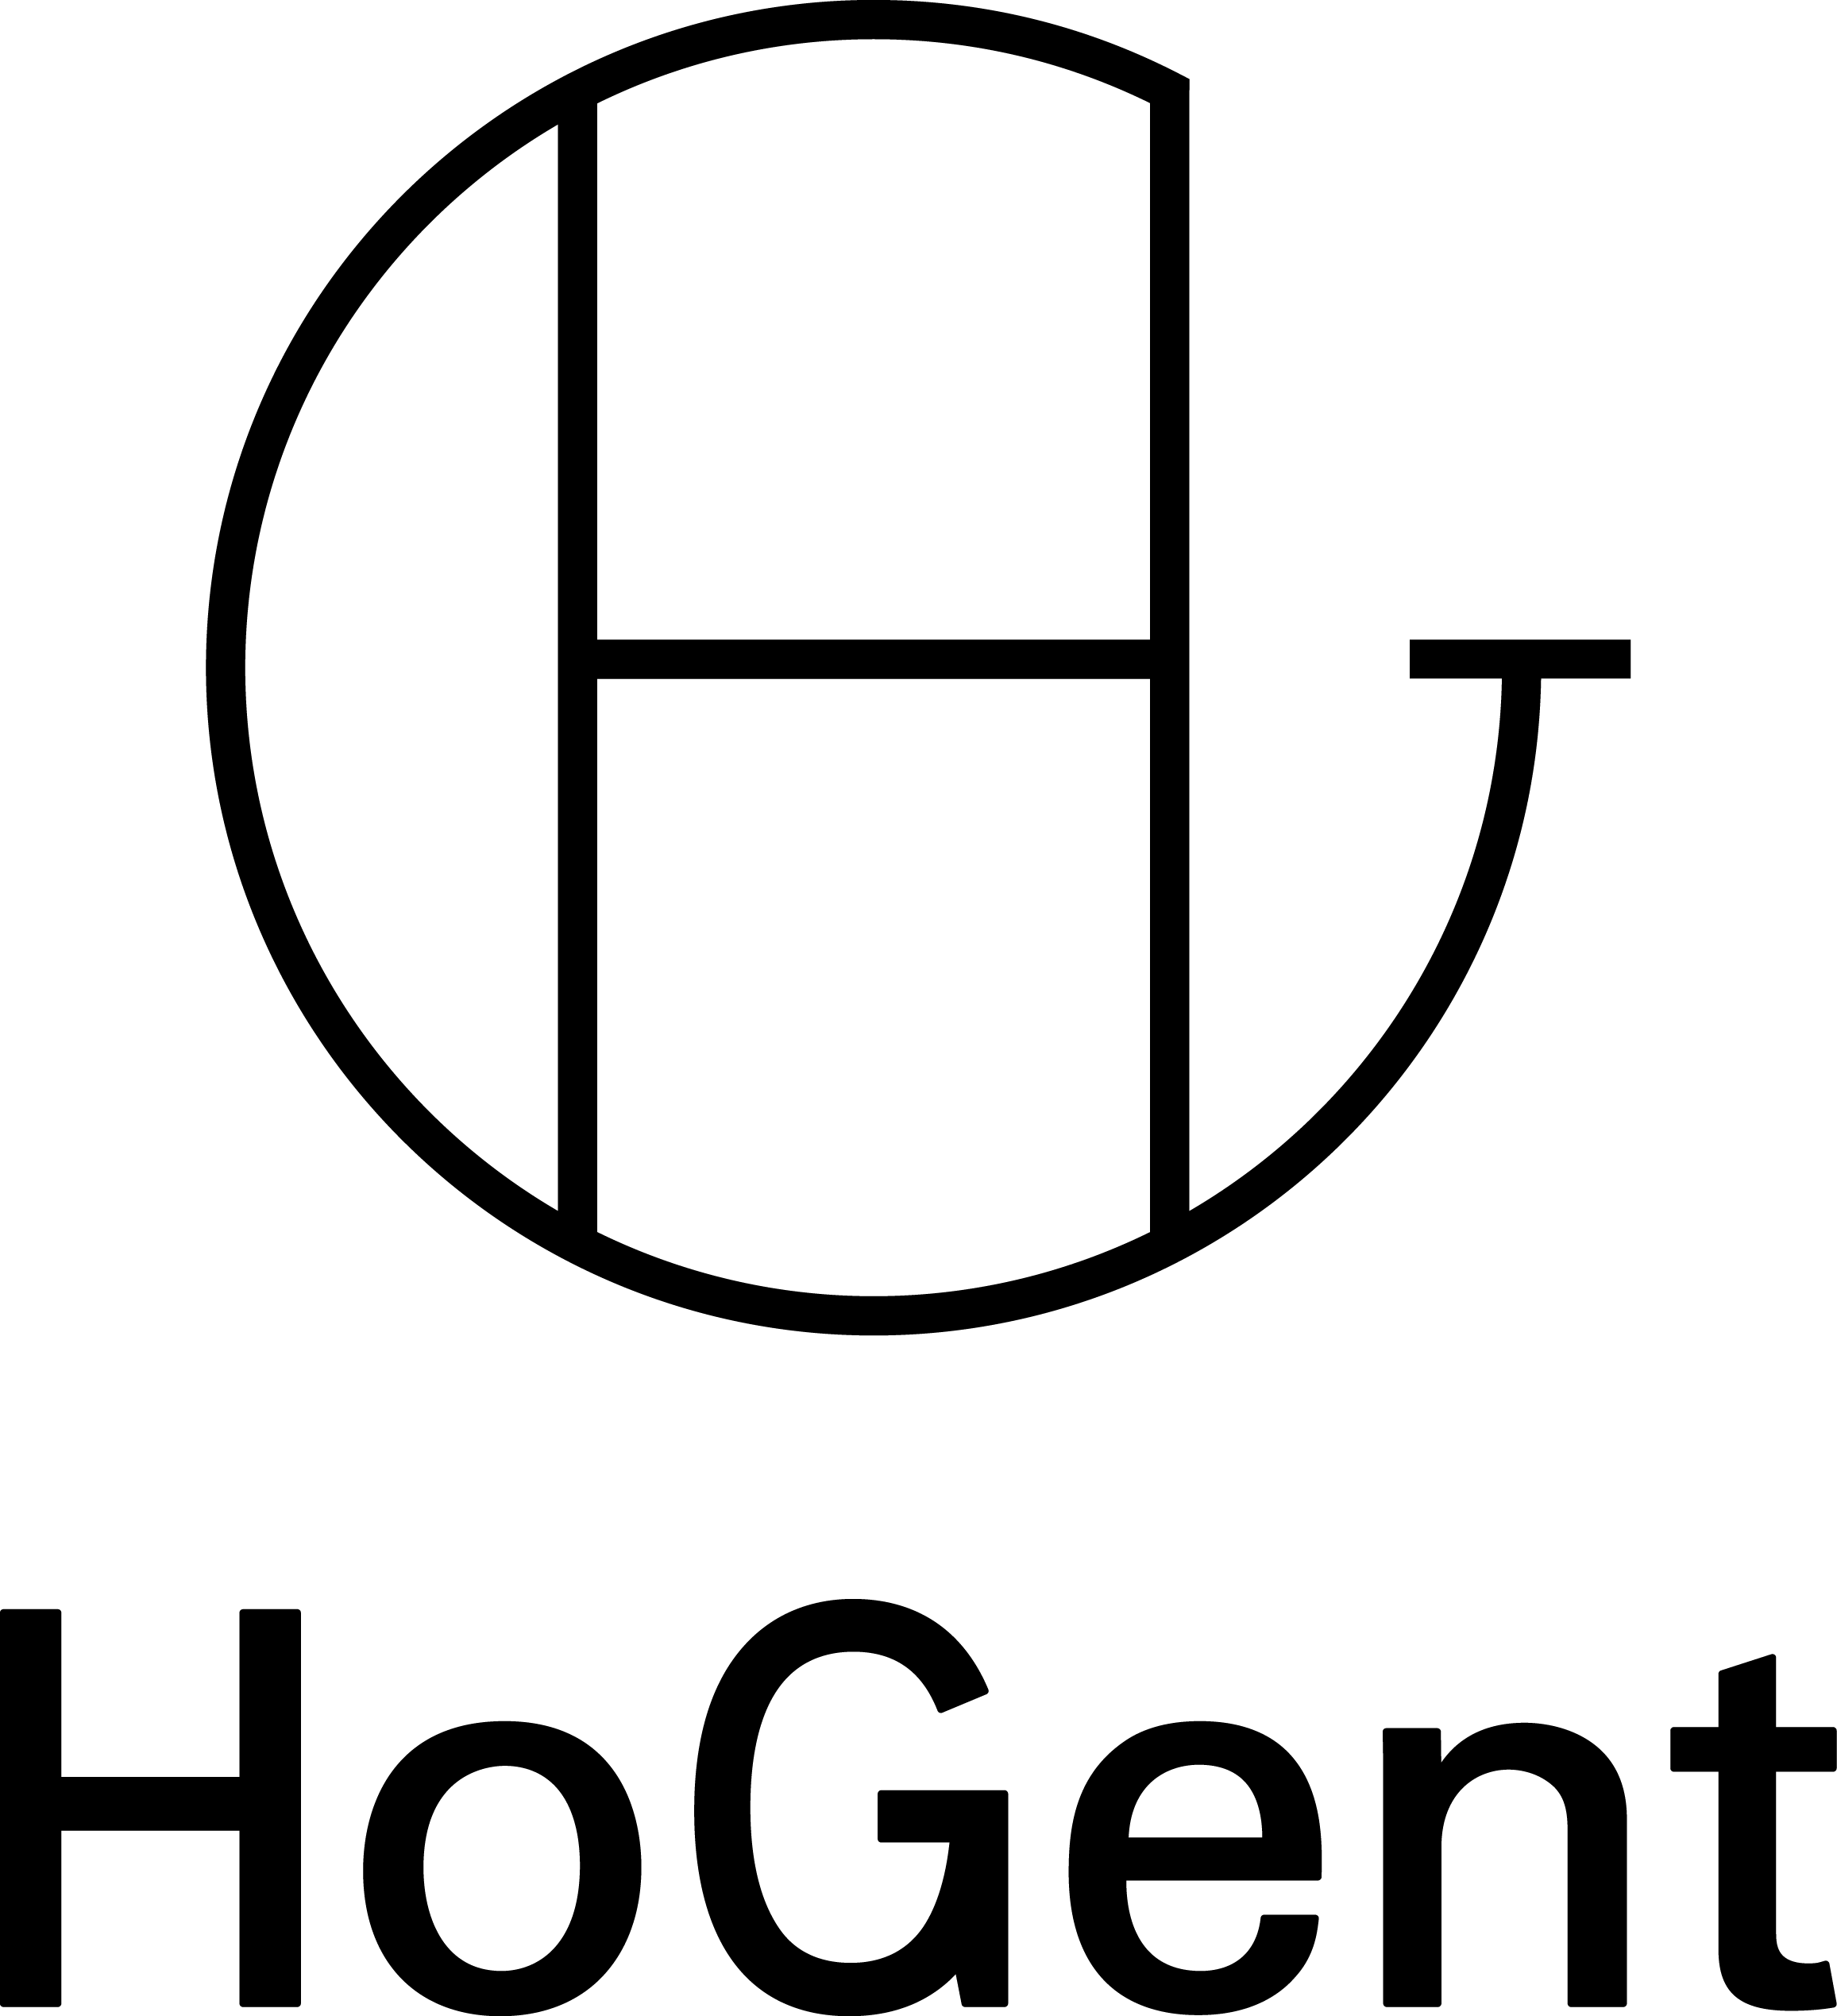
\includegraphics[width=2.5cm]{img/HG-beeldmerk-woordmerk}\\[.5cm]
    \faculteit\\[3cm]
    \titel
    \vfill
    \student\\[3.5cm]
    \rapporttype\\[2cm]
    Promotor:\\
    \promotor\\
    Co-promotor:\\
    \copromotor\\[2.5cm]
    Academiejaar: \academiejaar\\[.5cm]
    \examenperiode
    \endgroup

  \end{center}
  \restoregeometry
\end{titlepage}

% Schutblad

\emptypage


\begin{titlepage}
  \newgeometry{top=5.35cm,bottom=1.5cm,left=1.5cm,right=1.5cm}
  \begin{center}

    \begingroup
    \rmfamily
    \faculteit\\[3cm]
    \titel
    \vfill
    \student\\[3.5cm]
    \rapporttype\\[2cm]
    Promotor:\\
    \promotor\\
    Co-promotor:\\
    \copromotor\\[2.5cm]
    Academiejaar: \academiejaar\\[.5cm]
    \examenperiode
    \endgroup

  \end{center}
  \restoregeometry
\end{titlepage}


\begin{abstract}
% TODO: De "abstract" of samenvatting is een kernachtige (max 1 blz. voor een
% thesis) synthese van het document. In ons geval beschrijf je kort de
% probleemstelling en de context, de onderzoeksvragen, de aanpak en de
% resultaten.
 \subfile{sections/abstract}
\end{abstract}

\chapter*{Voorwoord}
\subfile{sections/voorwoord}

\tableofcontents

% Als je een lijst van afkortingen of termen wil toevoegen, dan hoort die
% hier thuis. Gebruik bijvoorbeeld de ``glossaries'' package.

%%---------- Kern --------------------------------------------------------
\chapter{Inleiding}
\subfile{sections/inleiding}

\chapter{Beschrijving van CMS}
\subfile{sections/cms}

\chapter{Voor wie is dit onderzoek bedoeld?}
\subfile{sections/doelpubliek}

\chapter{Pijnpunten Drupal CMS }
\subfile{sections/probs-drupal}


\chapter{Laravel}
\subfile{sections/laravel}

\chapter{Casus concreet definiëren}
\subfile{sections/casus}

\chapter{Methodologie}
\subfile{sections/methodologie}

\section{Drupal}
\subfile{methodologie/drupal}

\section{OctoberCMS}
\subfile{methodologie/octobercms}

\chapter{Vergelijkende testen en resultaat}
\subfile{sections/resultaten}

\chapter{Conclusie}
\subfile{sections/conclusie}

%%---------- Appendix -------------------------------------------------

\appendix
\chapter{Casus code - Github}
\label{AppendixCode}

Aan de hand van de vooropgestelde casus werd een site opgesteld voor beide systemen (Drupal en OctoberCMS).
\newline\newline
De code kan terug gevonden worden op GitHub, \newline 
via deze link: \hyperlink{https://github.com/DieterVyncke/BP}{https://github.com/DieterVyncke/BP}
\chapter{Casus - Designs}
\label{AppendixDesigns}

De casus bevat een voorgedefinieerde template die exact zal uitgewerkt worden in twee systemen. Beide systemen worden uitgetest op een bestaand design voor een bedrijfswebsite. Deze website bevat de meest typerende en meest belangrijke elementen als voorbeeld voor een CMS.

\begin{figure}[!ht]
  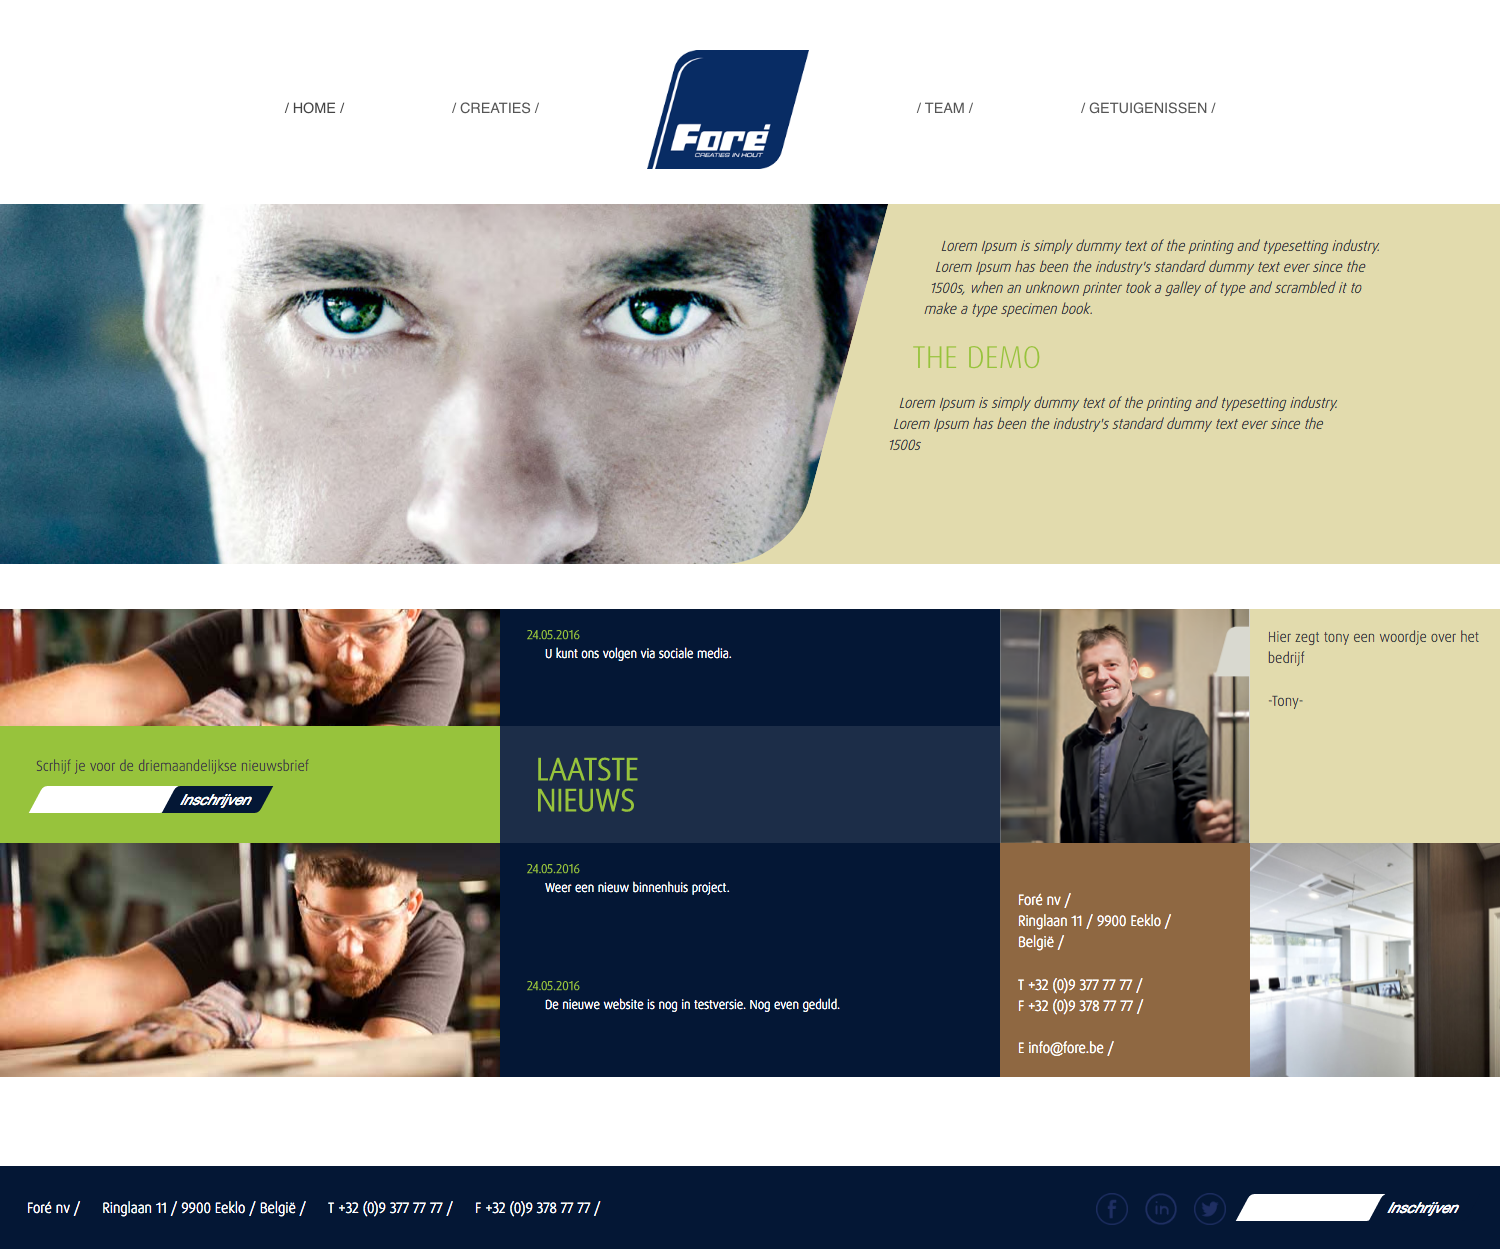
\includegraphics[width=110mm]{img/design-01.png}
  \centering
  \caption{Casus design homepagina}
  \label{fig:Casus design homepagina}
\end{figure}

\begin{figure}[!ht]
  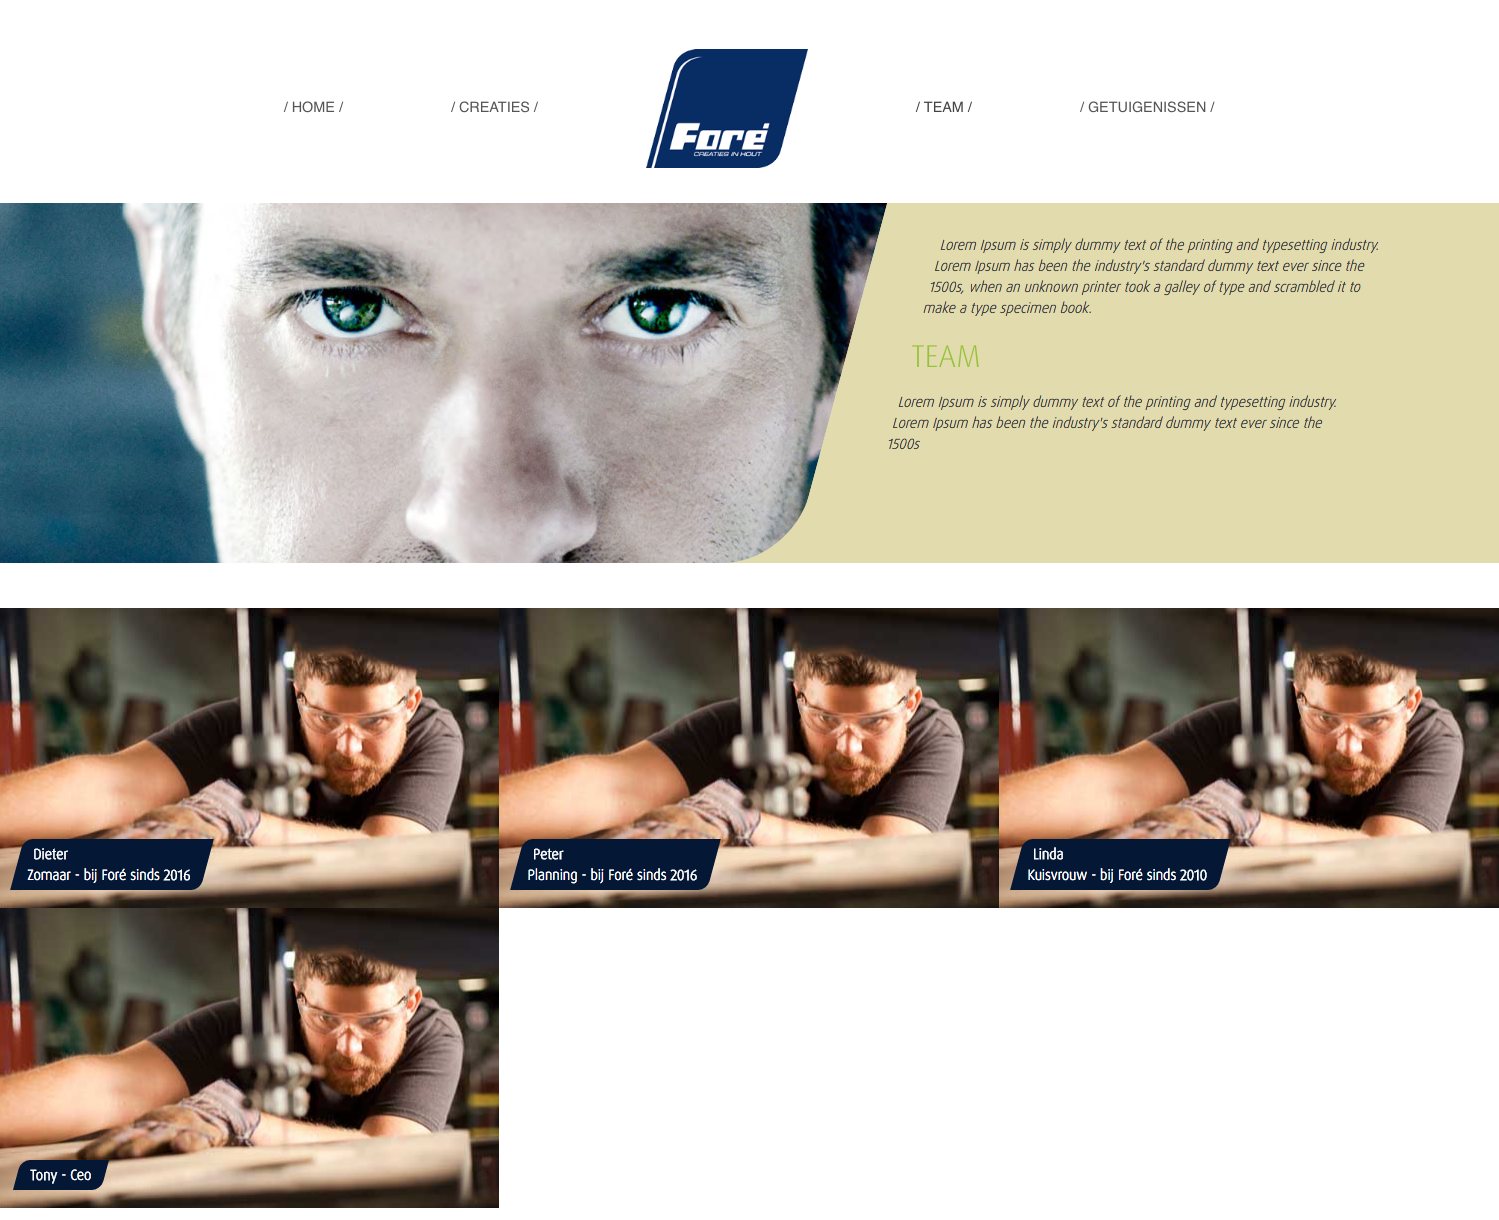
\includegraphics[width=110mm]{img/design-02.png}
  \centering
  \caption{Casus design team}
  \label{fig:Casus design team}
\end{figure}

\begin{figure}[!ht]
  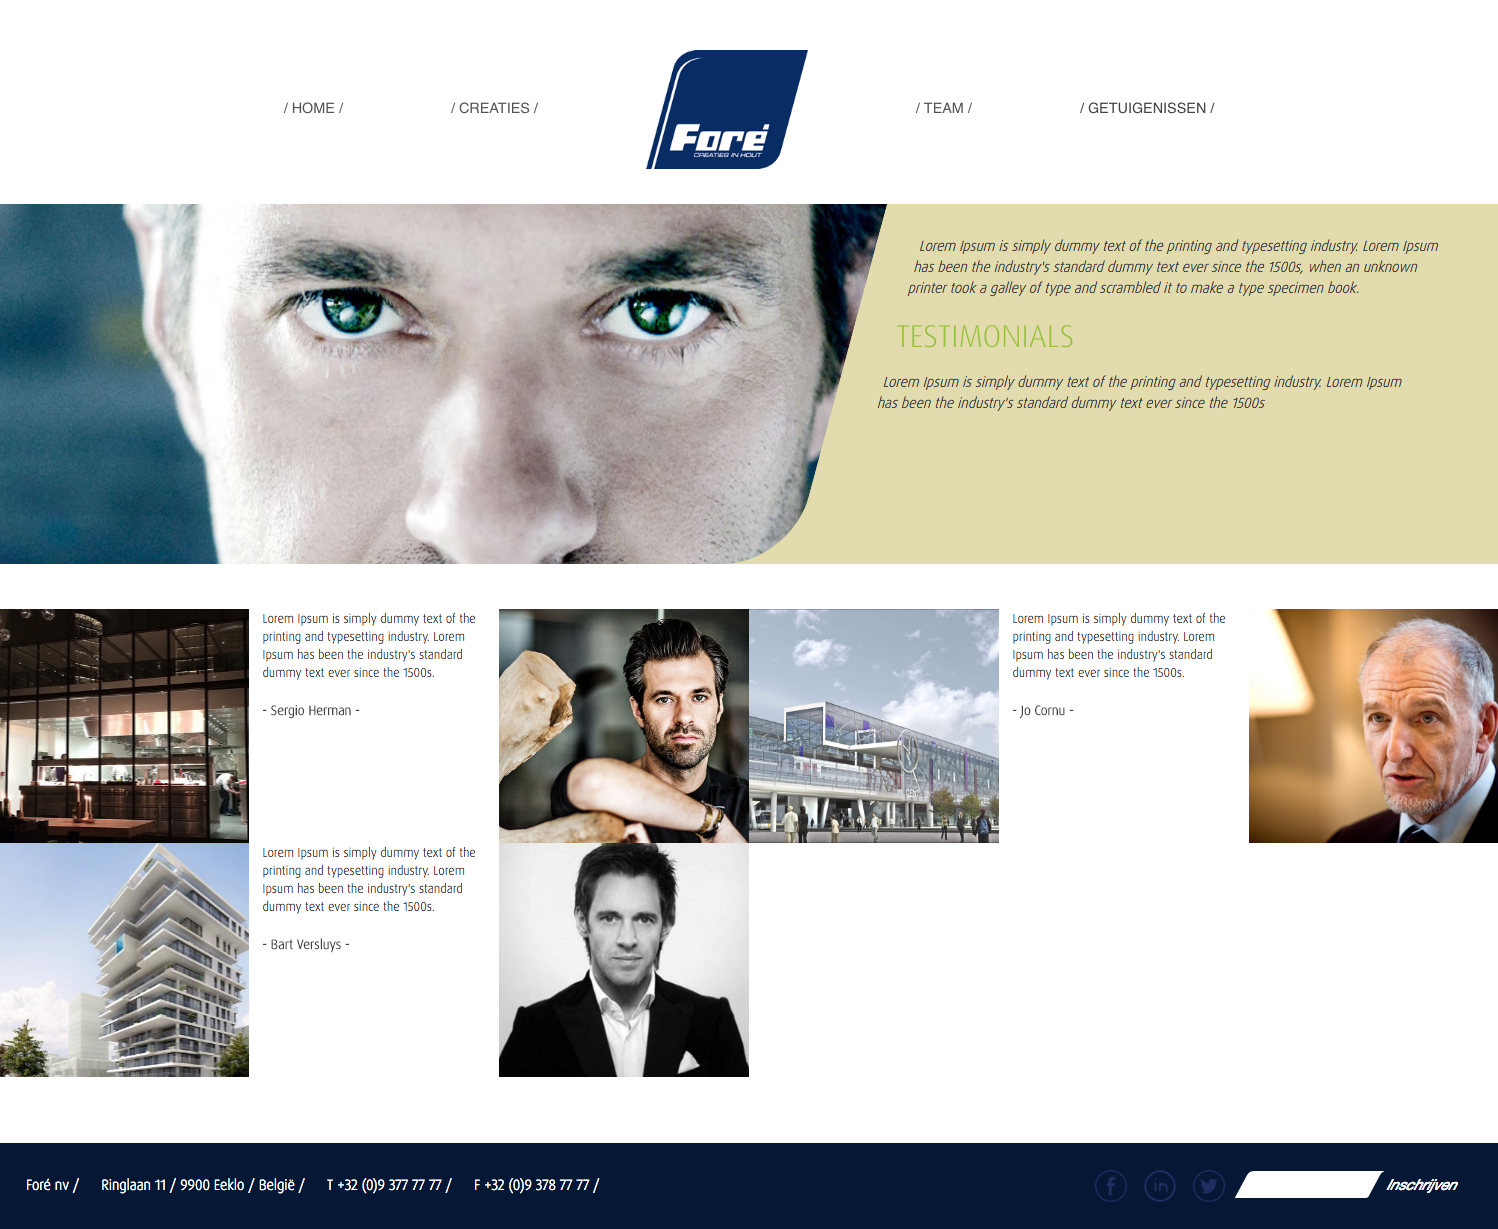
\includegraphics[width=110mm]{img/design-03.png}
  \centering
  \caption{Casus design testimonials}
  \label{fig:Casus design testimonials}
\end{figure}

\begin{figure}[!ht]
  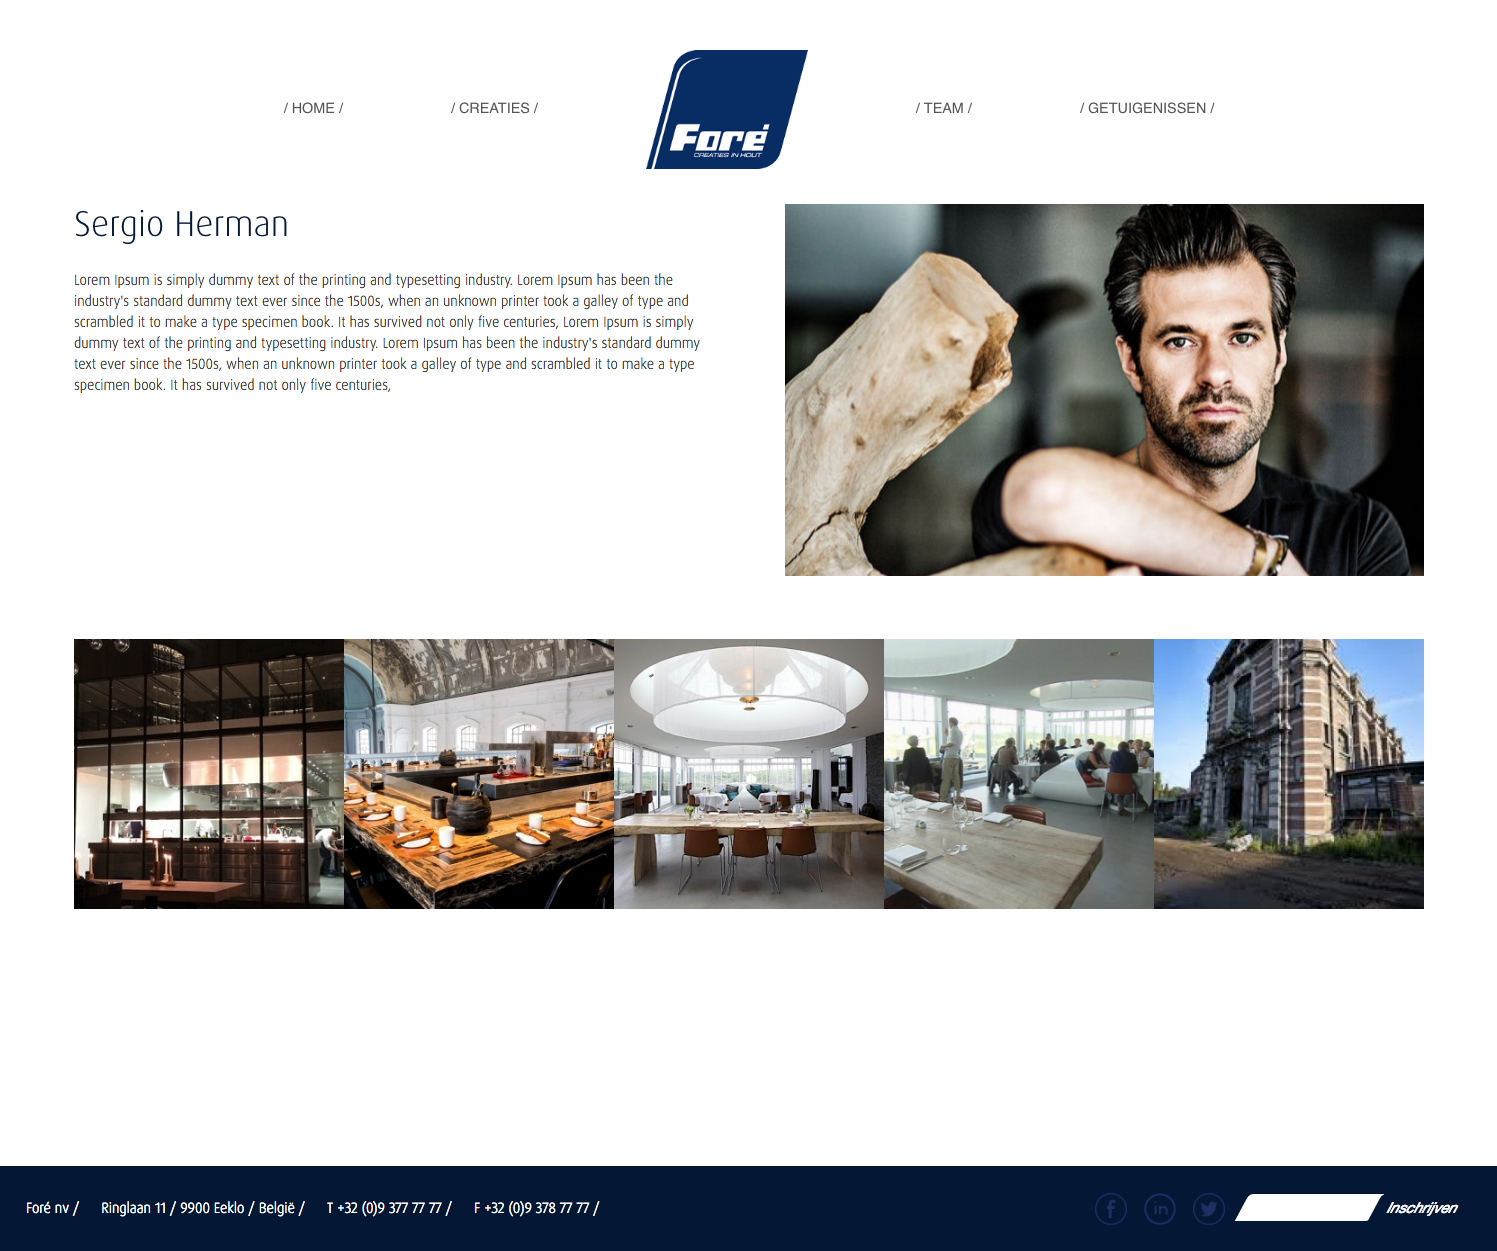
\includegraphics[width=110mm]{img/design-04.png}
  \centering
  \caption{Casus design testimonials detail}
  \label{fig:Casus design testimonials detail}
\end{figure}

\begin{figure}[!ht]
  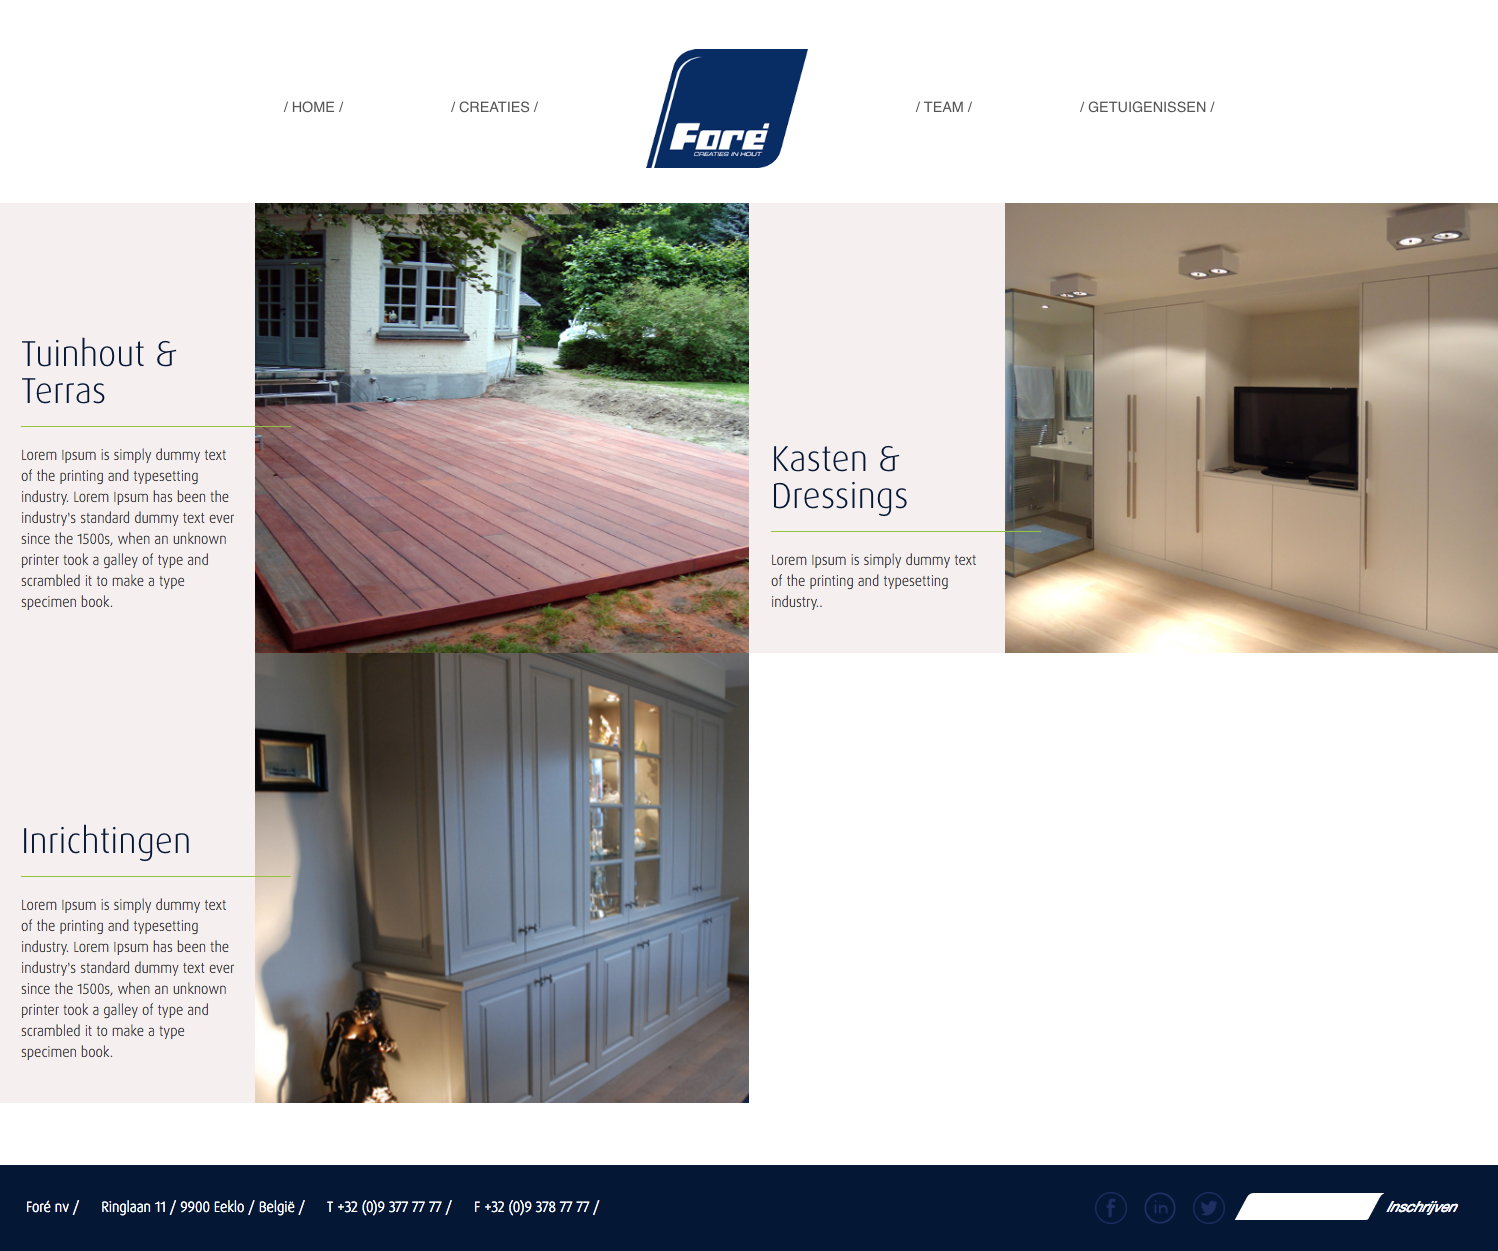
\includegraphics[width=110mm]{img/design-05.png}
  \centering
  \caption{Casus design categorie overzicht}
  \label{fig:Casus design categorie overzicht}
\end{figure}

\begin{figure}[!ht]
  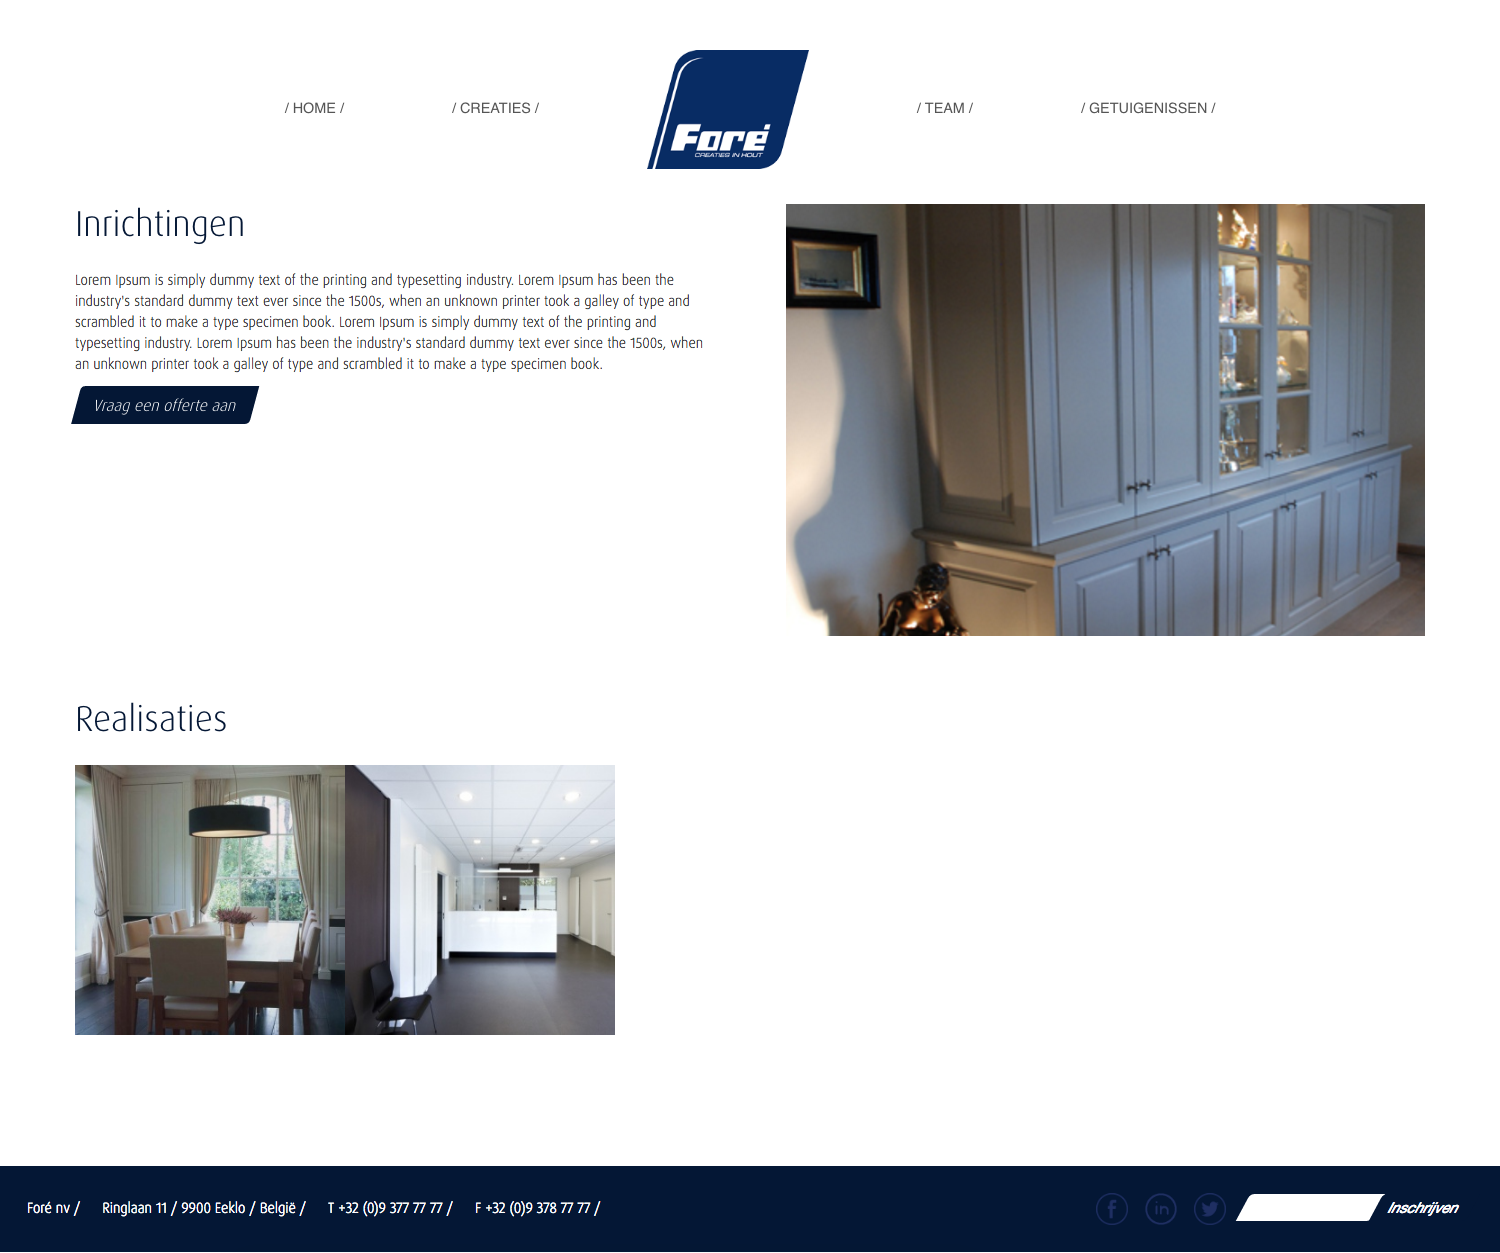
\includegraphics[width=110mm]{img/design-06.png}
  \centering
  \caption{Casus design categorie detail}
  \label{fig:Casus design categorie detail}
\end{figure}

\begin{figure}[!ht]
  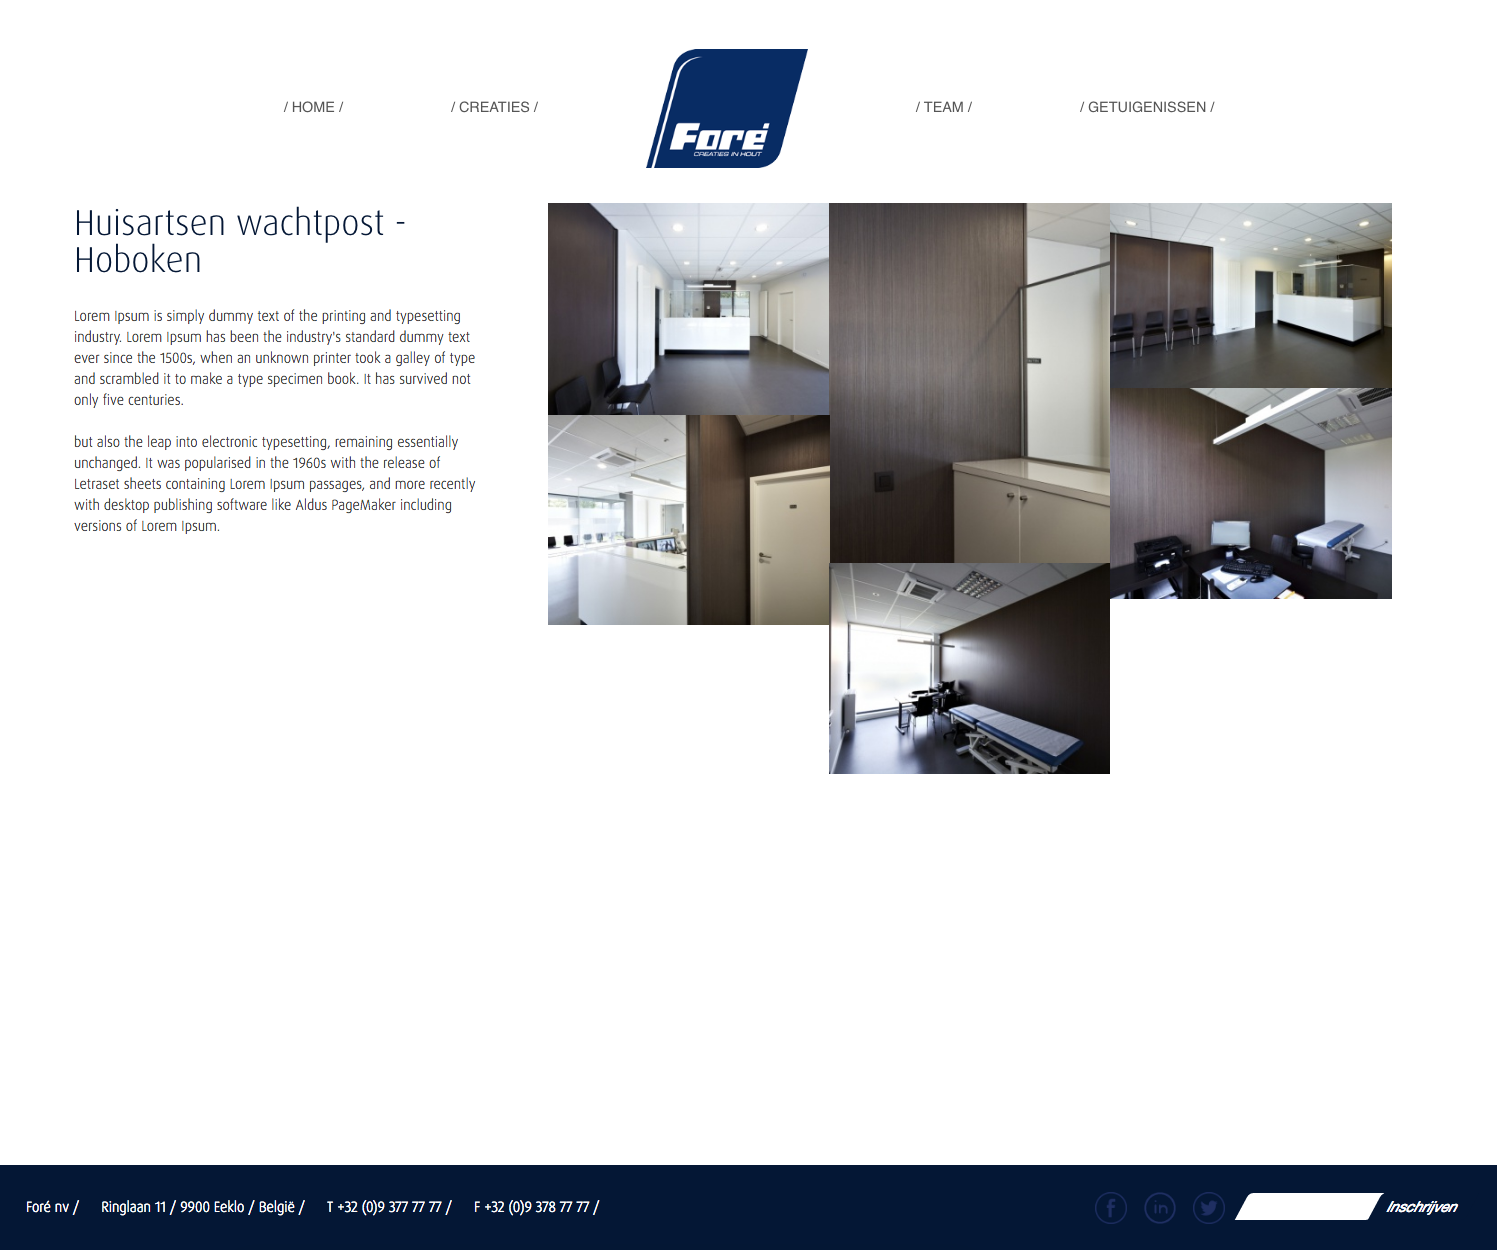
\includegraphics[width=110mm]{img/design-07.png}
  \centering
  \caption{Casus design realisatie}
  \label{fig:Casus design realisatie}
\end{figure}

\bibliographystyle{apa}
\bibliography{BP}

%%---------- Back matter -------------------------------------------------

\listoffigures
\listoftables

% Leeg blad
\emptypage

\end{document}
